\subsection*{問題4}
16進数の1F5Bを2進数,10進数にそれぞれ直せ.また,10進数の300を16進数,2進数にそれぞれ直せ.
$$
(1F5B)_{16}=(1111101011011)_2=(8027)_{10}
$$
$$
(300)_{10}=(12C)_{16}=(100101100)_2
$$

\subsection*{問題5}
$C_3-C_1<0$の場合,出力の2進数の2の補数を取ることにより,$|C_3-C_1|$の正の数が得られる
ことを計算により確認せよ.

$C_3$を0x55,$C_1$を0x08とすると出力は$(11111101)_2=(-3)_{10}$となった.
この出力の2の補数をとると$(00000011)_2=(3)_{10}$と求められる.よって,
$C_3-C_1<0$の時,2の補数をとると$|C_3-C_1|$の正の数が得られることができた.

\subsection*{問題6}
このFFはクロックの立ち上がりでDを取り込むポジティブエッジトリガ型か,
クロックの立ち下がりでDを取り込むネガティブエッジトリガ型のどちらか?

与えられたFFはポジティブエッジトリガ型である.

\subsection*{問題7}
クロック周波数を上げていくと,LEDの点滅が認識できず,点灯状態に見え
る.点灯状態に見える最低の周波数はいくらか?この周波数と,映画やテレビなどの
動画のフレームレートの関係を調べよ.

Cube-Dでの実験上では,点灯状態に見える最低の周波数は$70\mathrm{Hz}$であった.

一般的な映画やテレビのフレームレートは$50\mathrm{Hz}$以下になっている.
fpsが上がると動画が滑らかになる一方で,データ量が増えることから用途に
合った適切なフレームレートが決められていると考えられる.
\begin{figure}[H]
    \centering
    \caption{フレームレートの主な種類と一般的な用途}
    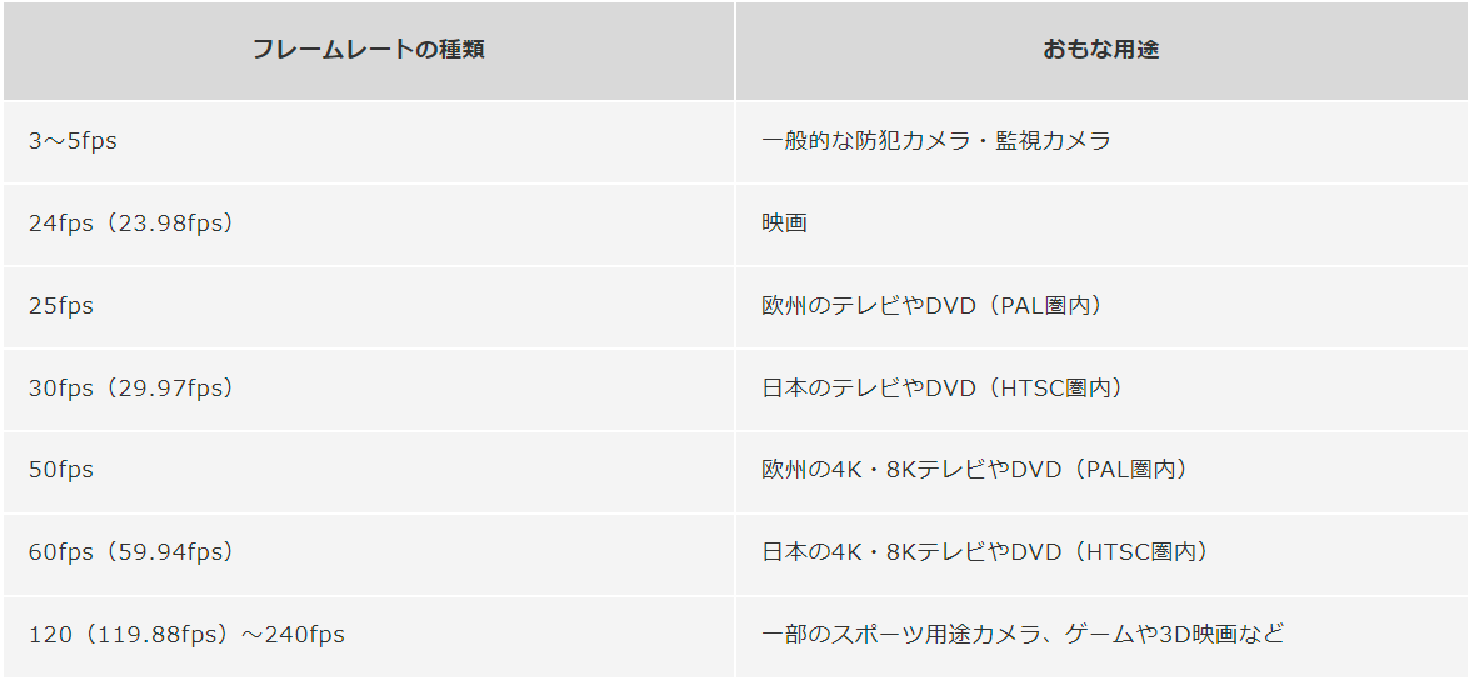
\includegraphics[scale=0.5]{figure2.pdf}
\end{figure} 

\subsection*{問題8}
フリップフロップのメタステーブルについて調べよ.

フリップフロップに入力されるデータ信号は,安定動作の要件としてクロックと入力信号の間に
セットアップタイムとホールドタイムなどのタイミング規定が設けられており,
クロックの立ち上がりのタイミングでセットアップタイムとホールドタイムで規定される期間以上に
安定している必要がある.この規定を守れない場合,フリップフロップの出力信号は一定期間発振した
状態になり,この状態をメタステーブルという. 
また,非同期入力についてはメタステーブルが発生しても,回路動作に影響を与えないよ
うフリップフロップを複数段配置することで対策する.

\subsection*{問題9}
1オクターブ上がると周波数はどのように変化するか.♯も含めて,ピアノの
鍵盤の隣接する音の関係を調べよ.

1オクターブ上がると周波数は倍になり,ピアノの鍵盤の隣接する音の関係は,
公比$r=\sqrt[12]{212}$の等比数列である.